\section{Architektur}
\begin{figure}[ht]
	\centering
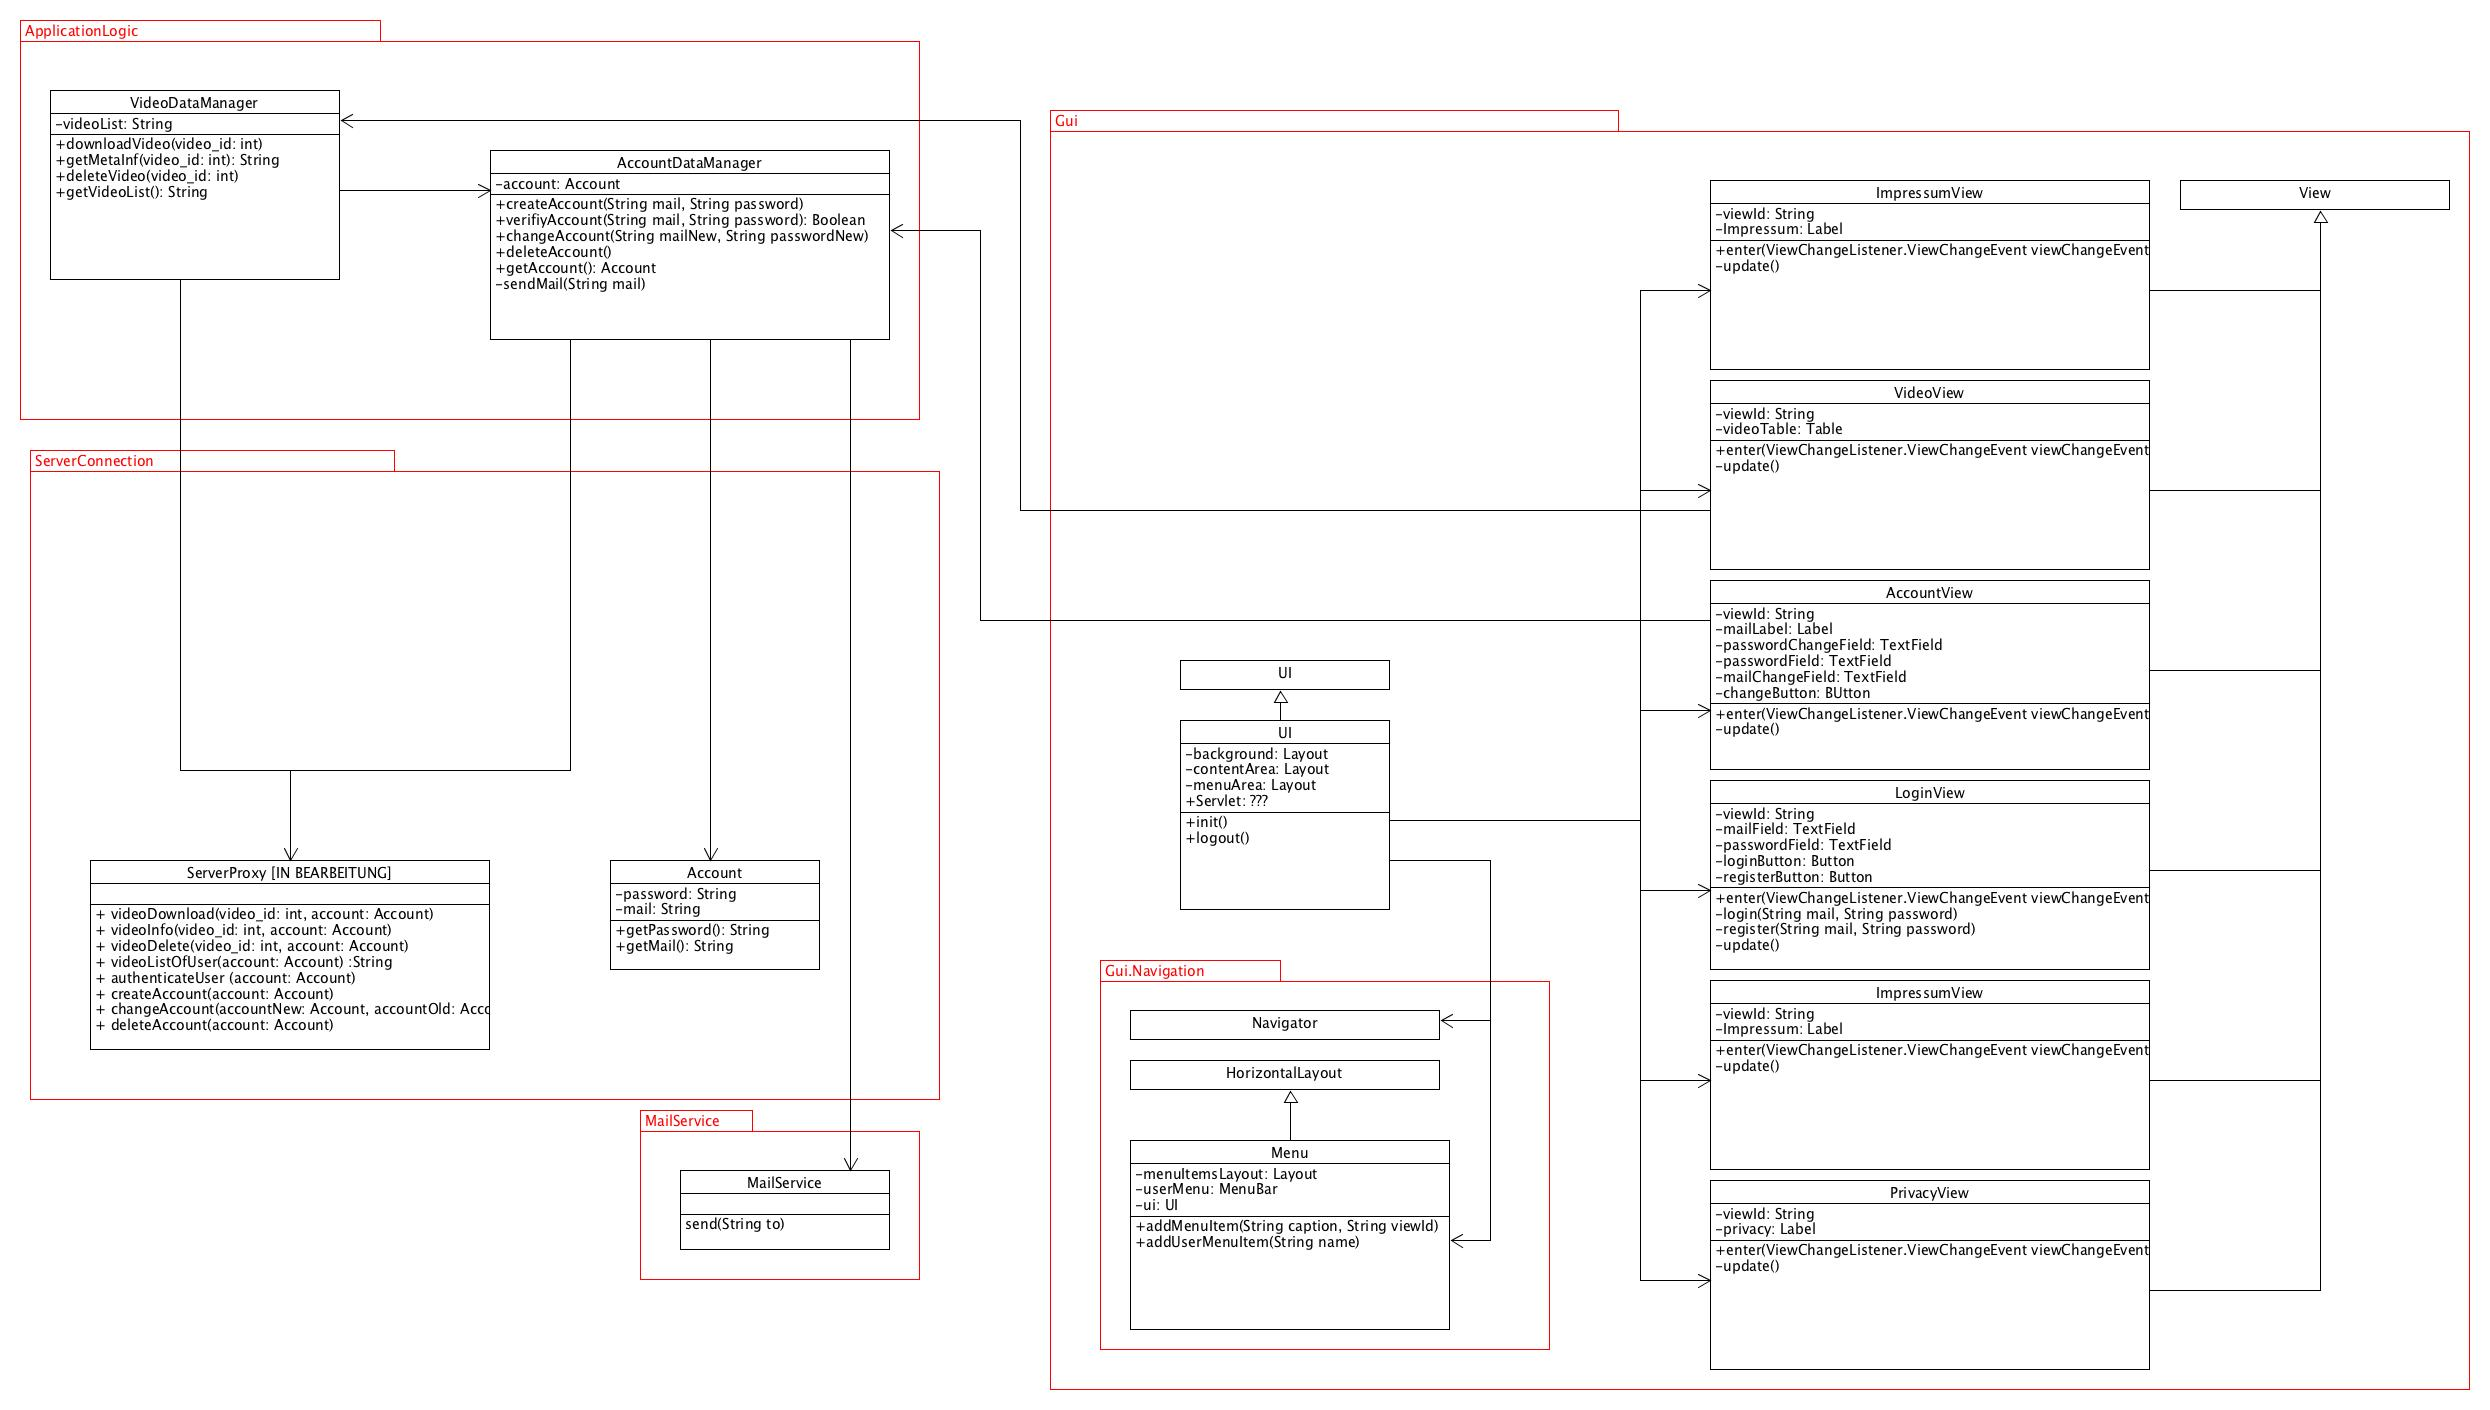
\includegraphics[width=1\textwidth]{./resources/Diagramme/WebInterface/UMLWebInterface.jpg}
\caption{UML Diagramm des Web-Interface}
	\label{interface:fig:modules_overview}
\end{figure}

\subsection{Entwurfsmuster}
Im Web-Interface wurden Entwurfsmuster verwendet um austauschbare Klassen zu erhalten. Zudem helfen sie dabei das hinzufügen neuer Funktionalität möglichst einfach zu gestalten, was bei der Umsetzung von Wunschkriterien durchaus von Bedeutung sein wird.

\subsubsection{Proxy}
Da die Datenmanager Daten vom Web-Dienst holen müssen, wurde hier ein Proxy, der ServerProxy, zwischengeschalten um den Zugriff zu regeln. Des Weiteren werden so die Klassen des DataManagement Moduls vom Web-Dienst Entkoppelt.

\subsubsection{Zustandsmuster}
Der Navigator verwendet ein Zustandsmuster um die Views anzuzeigen. Die verschiedenen Views entsprechen dabei den States.

\subsubsection{Schablonenmethode}
Die Klasse VideoDataManager verwendet eine Schablonenmethode zum erzeugen der Video Liste. In dieser werden die Videos und die Informationen vom Server geholt und dann entsprechend verarbeitet.
\newpage
